\documentclass[border=5pt]{standalone}
\usepackage{tikz}
\usepackage{xcolor}

\definecolor{Garnet}{HTML}{73000A}

\tikzset{every node/.append style={rounded corners=0pt}}

\begin{document}
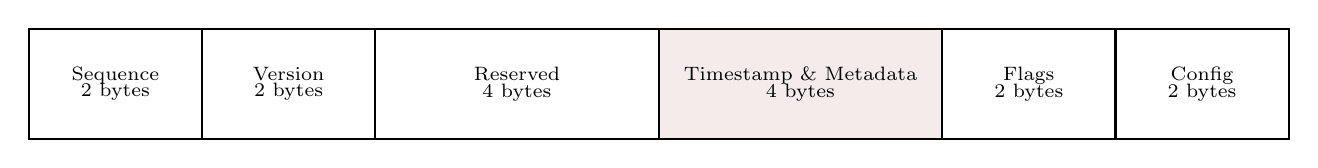
\begin{tikzpicture}[
    block/.style={draw, thick, minimum height=1.4cm, anchor=west, align=center, fill=white, font=\scriptsize},
]

\node[block, minimum width=2.2cm] at (0, 0) {Sequence\\[-2pt]2 bytes};
\node[block, minimum width=2.2cm] at (2.2, 0) {Version\\[-2pt]2 bytes};
\node[block, minimum width=3.6cm] at (4.4, 0) {Reserved\\[-2pt]4 bytes};
\node[block, minimum width=3.6cm, fill=Garnet!8] at (8.0, 0) {Timestamp \& Metadata\\[-2pt]4 bytes};
\node[block, minimum width=2.2cm] at (11.6, 0) {Flags\\[-2pt]2 bytes};
\node[block, minimum width=2.2cm] at (13.8, 0) {Config\\[-2pt]2 bytes};

\end{tikzpicture}
\end{document}
